%%%%%%%% ICML 2018 EXAMPLE LATEX SUBMISSION FILE %%%%%%%%%%%%%%%%%

\documentclass{article}

% Recommended, but optional, packages for figures and better typesetting:
\usepackage{microtype}
\usepackage{graphicx}
\usepackage{subfigure}
\usepackage{booktabs} % for professional tables

% hyperref makes hyperlinks in the resulting PDF.
% If your build breaks (sometimes temporarily if a hyperlink spans a page)
% please comment out the following usepackage line and replace
% \usepackage{icml2018} with \usepackage[nohyperref]{icml2018} above.
\usepackage{hyperref}

% Attempt to make hyperref and algorithmic work together better:
\newcommand{\theHalgorithm}{\arabic{algorithm}}

% Use the following line for the initial blind version submitted for review:
\usepackage{icml2018}
\usepackage{natbib}
\usepackage{amsmath}
\usepackage{amsthm}
\usepackage{amsfonts}
\usepackage{bbm}
\usepackage{bm}
\usepackage{amssymb}
\usepackage{enumitem}
\newtheorem{theorem}{Theorem}
\newtheorem{proposition}[theorem]{Proposition}
\newtheorem{definition}{Definition}
\newtheorem{lemma}[theorem]{Lemma}
\setcounter{theorem}{2}
%\makeatletter
%\renewenvironment{proof}[1][\proofname]{\par
%  \vspace{-\topsep}% remove the space after the theorem
%  \pushQED{\qed}%
%  \normalfont
%  \topsep0pt \partopsep0pt % no space before
%  \trivlist
%  \item[\hskip\labelsep
%        \itshape
%    #1\@addpunct{.}]\ignorespaces
%}{%
%  \popQED\endtrivlist\@endpefalse
%  \addvspace{0pt plus 0pt} % some space after
%}
%\makeatother

% If accepted, instead use the following line for the camera-ready submission:
%\usepackage[accepted]{icml2018}

% The \icmltitle you define below is probably too long as a header.
% Therefore, a short form for the running title is supplied here:
\usepackage{xr-hyper}
\externaldocument[MF-]{main}
\icmltitlerunning{Supplementary File}

\renewcommand{\thesection}{\Alph{section}}
\setcounter{equation}{20}

\begin{document}

\twocolumn[
\icmltitle{Appendix for ``Inference Aided Reinforcement Learning for \\
Incentive Mechanism Deisgn in Crowdsourcing"} 

% It is OKAY to include author information, even for blind
% submissions: the style file will automatically remove it for you
% unless you've provided the [accepted] option to the icml2018
% package.

% List of affiliations: The first argument should be a (short)
% identifier you will use later to specify author affiliations
% Academic affiliations should list Department, University, City, Region, Country
% Industry affiliations should list Company, City, Region, Country

% You can specify symbols, otherwise they are numbered in order.
% Ideally, you should not use this facility. Affiliations will be numbered
% in order of appearance and this is the preferred way.
\icmlsetsymbol{equal}{*}

\begin{icmlauthorlist}
\icmlauthor{Zehong Hu}{NTU}
\icmlauthor{Yang Liu}{Harvard}
\icmlauthor{Yitao Liang}{UCLA}
\icmlauthor{Jie Zhang}{NTU}
\end{icmlauthorlist}

%\icmlaffiliation{NTU}{Rolls-Royce Cooperate Lab@NTU, School of Computer Science and Engineering, Nanyang Technological University, Singapore}
%\icmlaffiliation{goo}{Googol ShallowMind, New London, Michigan, USA}
%\icmlaffiliation{ed}{School of Computation, University of Edenborrow, Edenborrow, United Kingdom}

%\icmlcorrespondingauthor{Cieua Vvvvv}{c.vvvvv@googol.com}
%\icmlcorrespondingauthor{Eee Pppp}{ep@eden.co.uk}

% You may provide any keywords that you
% find helpful for describing your paper; these are used to populate
% the "keywords" metadata in the PDF but will not be shown in the document
%\icmlkeywords{Machine Learning, ICML}

\vskip 0.3in
]

% this must go after the closing bracket ] following \twocolumn[ ...

% This command actually creates the footnote in the first column
% listing the affiliations and the copyright notice.
% The command takes one argument, which is text to display at the start of the footnote.
% The \icmlEqualContribution command is standard text for equal contribution.
% Remove it (just {}) if you do not need this facility.

%\printAffiliationsAndNotice{}  % leave blank if no need to mention equal contribution
%\printAffiliationsAndNotice{} % otherwise use the standard text.
\section{Background for Reinforcement Learning}
In this section, we introduce some important concepts about reinforcement learning (RL). In an RL problem, an agent interacts with an unknown environment and attempts to maximize its cumulative collected reward \citep{Sutton98,Szepesvari10}. The environment is commonly formalized as a Markov Decision Process (MDP) defined as $\mathcal{M} = \langle \mathcal{S}, \mathcal{A}, \mathcal{R}, \mathcal{P}, \gamma\rangle$. At time $t$ the agent is in state $s_t \in \mathcal{S}$ where it takes an action $a_t \in \mathcal{A}$ leading to the next state $s_{t+1} \in \mathcal{S}$ according to the transition probability kernel $\mathcal{P}$, which encodes $\mathbb{P}(s_{t+1}\mid s_t,a_t)$. In most RL problems, $\mathcal{P}$ is unknown to the agent. The agent's goal is to learn the optimal policy, a conditional distribution $\pi(a \mid s)$ that  maximizes the sate's value function. The value function calculates the cumulative reward the agent is expected to receive given it would follow the current policy $\pi$ after observing the current state $s_t$
$$
V^\pi(s) = \mathbb{E}_\pi \left[ \sum_{k=1}^\infty \gamma^k r_{t+k} \mid s_t = s   \right].
$$
Intuitively, it measures how preferable each state is given the current policy.

As a critical step towards improving a given policy, it is a standard practice for RL algorithms to learn a state-action value function (i.e. Q-function). Q-function calculates the expected cumulative reward if agent choose $a$ in the current state and follows $\pi$ thereafter
\begin{equation*}
\begin{split}
&Q^\pi(s,a) =\\
& \quad\mathbb{E}_\pi\left[ \mathcal{R}(s_t,a_t,s_{t+1}) + \gamma V^\pi(s_{t+1}) \mid s_t = s, a_t = a \right].
\end{split}
\end{equation*}
In real-world problems, in order to achieve better generalization, instead of learning a value for each state-action pair, it is more common to learn an approximate value function: $Q^\pi(s,a; \theta) \approx Q^\pi(s,a)$. A standard approach is to learn a feature-based state representation $\phi(s)$ instead of using the raw state $s$ \citep{Gordon00}. Due to the popularity of Deep Reinforcement learning, it has been a trend to deploy neural networks to automatically extract high-level features \citep{Silver17,Mnih15}. However, running most deep RL models are very computationally heavy. On contrast, static feature representations are usually light-weight and simple to deploy. Several studies also reveal that a carefully designed static feature representation can achieve performance as good as the most sophisticated deep RL models, even in the most challenging domains \citep{Liang16}.



\section{Basic Lemmas}
We firstly present some lemmas for our proof later.
\begin{lemma}
\label{MoGene}
If $x\sim \mathrm{Bin}(n,p)$, $\mathbb{E}t^x= \left(1-p+tp\right)^{n}$ holds for any $t>0$, where $\mathrm{Bin}(\cdot)$ is the binomial distribution.
\begin{proof}
\begin{equation}
t^x = e^{x\log t}=m_x(\log t)= \left(1-p+pe^{\log t}\right)^{n}
\end{equation}
where $m_x(\cdot)$ denotes the moment generating function.
\end{proof}
\end{lemma}

\begin{lemma}
\label{SolveF}
For given $n,m\geq 0$, if $0\leq p\leq 1$, we can have
\begin{equation*}
\begin{split}
&{\sum}_{x=0}^{n}{\sum}_{w=0}^{m} C_{n}^{x}C_{m}^{w}p^{x+w}(1-p)^{y+z}\times\\
&\qquad\qquad\qquad B(x+z+1+t,y+w+1)=\\
&\int_{0}^{1}[(2p-1)x+1-p]^{n}[(1-2p)x+p]^{m}x^{t}\mathrm{d}x
\end{split}
\end{equation*}
\begin{proof}
By the definition of the beta function~\cite{olver2010nist},
\begin{equation}
B(x, y) = \int_{0}^{+\infty} u^{x-1}(1+u)^{-(x+y)}\mathrm{d}u
\end{equation}
we can have
\begin{align}
&\sum_{x,w} C_{n}^{x}C_{m}^{w}p^{x+w}(1-p)^{y+z}B(x+z+1+t,y+w+1)\nonumber\\
&= \int_{0}^{+\infty} \mathbb{E}u^{x}\cdot\mathbb{E}u^z \cdot u^t\cdot (1+u)^{-(n+m+2+t)}\mathrm{d}u
\end{align}
where we regard $x\sim \mathrm{Bin}(n,p)$ and $z\sim \mathrm{Bin}(m,1-p)$.
Thus, according to Lemma~\ref{MoGene}, we can obtain
\begin{equation}
\begin{split}
&\int_{0}^{+\infty} \mathbb{E}u^{x}\cdot\mathbb{E}u^z \cdot u^t\cdot (1+u)^{-(n+m+3)}\mathrm{d}u\\
&=\int_{0}^{+\infty} \frac{[1-p+up]^n\cdot [p+(1-p)u]^m\cdot u^t}{(1+u)^{n+m+2+t}}\mathrm{d}u.
\end{split}
\end{equation}
For the integral operation, substituting $u$ with $v-1$ at first and then $v$ with $(1-x)^{-1}$, we can conclude Lemma~\ref{SolveF}.
\end{proof}
\end{lemma}

\begin{lemma}
\label{Sum1}
$\sum_{n=0}^{N}C_N^{n}\cdot x^{n}=(1+x)^N$.
\end{lemma}
\begin{lemma}
\label{Sum2}
$\sum_{n=0}^{N} C_N^{n}\cdot n\cdot x^{n}=N\cdot x\cdot (1+x)^{N-1}$.
\end{lemma}
\begin{lemma}
\label{Sum3}
$\sum_{n=0}^{N} C_N^{n}\cdot n\cdot x^{N-n}=N\cdot (1+x)^{N-1}$.
\end{lemma}
\begin{lemma}
\label{Sum5}
$\sum_{n=0}^{N} C_N^{n}\cdot n^2\cdot x^{n}=Nx(1+Nx)(1+x)^{N-2}$.
\end{lemma}
\begin{lemma}
\label{Sum6}
$\sum_{n=0}^{N} C_N^{n}\cdot n^2\cdot x^{N-n}=N(x+N)(1+x)^{N-2}$.
\end{lemma}
\begin{lemma}
\label{Sum4}
If $0<x<1$, we can have
\begin{equation*}
\begin{split}
\sum_{n=0}^{\lfloor N/2\rfloor} C_N^{n}\cdot x^{n} &\geq \left(1-e^{-cN}\right) \cdot (1+x)^{N}\\
\sum_{n=\lfloor N/2 \rfloor +1}^{N} C_N^{n}\cdot x^{N-n}&\geq \left(1-e^{-cN}\right) \cdot (1+x)^{N}.
\end{split}
\end{equation*}
where $c=0.5(1-x)^2(1+x)^{-2}$.
\begin{proof}
To prove the lemmas above, we firstly define
\begin{equation}
F_t(x)=\sum_{n=0}^{N} C_N^{n} n^t x^{n}
\end{equation}
Then, Lemma~\ref{Sum1} can be obtained by expanding $(1+x)^N$.
Lemma~\ref{Sum2} can be proved as follows
\begin{equation}
\begin{split}
F_1(x)&=\sum_{n=0}^{N} C_N^{n} (n+1) x^{n}-(1+x)^N\\
\sum_{n=0}^{N} C_N^{n} (n+1) x^{n}&=\frac{\mathrm{d}}{\mathrm{d}x}\left[xF_0(x)\right]\\
&=Nx(1+x)^{N-1}+(1+x)^N.
\end{split}
\end{equation}
Lemma~\ref{Sum3} can be obtained as follows
\begin{equation}
\begin{split}
\sum_{n=0}^{N} C_N^{n} n x^{N-n}&=x^N\sum_{n=0}^{N} C_N^{n} n \left(\frac{1}{x}\right)^n\\
&=x^N\cdot N\cdot \frac{1}{x}\cdot \left(1+\frac{1}{x}\right)^{N-1}.
\end{split}
\end{equation}
For Lemma~\ref{Sum5}, we can have
\begin{align}
F_2(x)&=\sum_{n=0}^{N} C_N^{n} (n+2)(n+1) x^{n}-3F_{1}(x)-2F_{0}(x)\nonumber \\
&=\left[x^2F_0(x)\right]' -3F_{1}(x)-2F_{0}(x)
\end{align}
Thus, we can have
\begin{equation}
F_2(x)=Nx(1+Nx)(1+x)^{N-2}
\end{equation}
which concludes Lemma~\ref{Sum5}.
Then, Lemma~\ref{Sum6} can be obtained by considering Equation~\ref{Eqv}.
\begin{equation}
\label{Eqv}
\begin{split}
\sum_{n=0}^{N} C_N^{n} n^2 x^{N-n}=x^N\sum_{n=0}^{N} C_N^{n} n^2 \left(\frac{1}{x}\right)^n.
\end{split}
\end{equation}
For Lemma~\ref{Sum4}, we can have
\begin{equation}
\sum_{n=0}^{\lfloor N/2\rfloor} C_N^{n} x^{n}=(1+x)^{N}\sum_{n=0}^{\lfloor N/2\rfloor} C_N^{n} p^n (1-p)^{N-n}
\end{equation}
where $p=x(1+x)^{-1}$. Let $X\sim \mathrm{Bin}(N, p)$, we can have
\begin{equation}
\sum_{n=0}^{\lfloor N/2\rfloor} C_N^{n} p^n (1-p)^{N-n}\geq 1-P\left(X\geq N/2\right).
\end{equation}
Since $x<1$, $p<0.5$ and $Np<N/2$. Considering Hoeffding's inequality, we can get
\begin{equation}
P\left(X\geq N/2\right)\leq \exp \left[-\frac{N(1-x)^2}{2(1+x)^2}\right]
\end{equation}
which concludes the first inequality in Lemma~\ref{Sum4}. Similarly, for the second inequality, we can have
\begin{equation}
\sum_{n=K}^{N} C_N^{n}x^{N-n}=(1+x)^{N}\sum_{n=K}^{N} C_N^{n} (1-p)^n p^{N-n}
\end{equation}
where $K=\lfloor N/2 \rfloor +1$. Suppose $Y\sim \mathrm{Bin}(N, 1-p)$, we can have
\begin{equation}
\sum_{n=K}^{N} C_N^{n} (1-p)^n p^{N-n}\geq 1-P\left(Y\leq N/2\right).
\end{equation}
Considering Hoeffding's inequality, we can also get
\begin{equation}
P\left(Y\leq N/2\right)\leq \exp \left[-\frac{N(1-x)^2}{2(1+x)^2}\right]
\end{equation}
which concludes the second inequality in Lemma~\ref{Sum4}.
\end{proof}
\end{lemma}

\begin{lemma}
\label{Inequality1}
For any $x,y\geq 0$, we can have
$$(1+x)^{y}\leq e^{xy}.$$
\begin{proof}
Firstly, we can know $(1+x)^{y}=e^{y\log(1+x)}$. Let $f(x)=x-\log(x)$. Then, we can have $f(0)=0$ and $f'(x)\geq 0$. Thus, $x\geq\log (1+x)$ and we can conclude Lemma~\ref{Inequality1} by taking this inequality into the equality.
\end{proof}
\end{lemma}

\begin{lemma}
\label{Concave1}
$$g(x)=\frac{e^x}{e^x+1}$$
is a concave function when $x\in [0,+\infty)$.
\begin{proof}
$g'(x)= (2+t(x))^{-1}$, where $t(x)=e^x+e^{-x}$. $t'(x)=e^x-e^{-x}\geq 0$ when $x\in [0,+\infty)$. Thus, $g'(x)$ is monotonically decreasing when $x\in [0,+\infty)$, which concludes Lemma~\ref{Concave1}.
\end{proof}
\end{lemma}

\begin{lemma}
\label{Concave2}
For $x\in(-\infty, +\infty)$, 
$$h(x)=\frac{1}{e^{|x|}+1}$$
satisfies
$$h(x)< e^x \;\;\mathrm{and}\;\; h(x)< e^{-x}.$$
\begin{proof}
When $x\geq 0$, we can have
\begin{equation}
h(x)<\frac{1}{e^x}=e^{-x}\leq e^{x}.
\end{equation}
When $x\leq 0$, we can have
\begin{equation}
h(x)=\frac{e^x}{e^x+1}<e^{x}\leq e^{-x}.
\end{equation}
\end{proof}
\end{lemma}

\begin{lemma}
\label{Concave3}
If $\lambda=p/(1-p)$ and $0.5<p<1$, then
$${\sum}_{n=\lfloor N/2 \rfloor}^{N}C_N^n\lambda^{m-n}p^n(1-p)^m\leq [4p(1-p)]^{N/2}$$
$${\sum}_{n=0}^{\lfloor N/2 \rfloor}C_N^n\lambda^{n-m}p^n(1-p)^m\leq [4p(1-p)]^{N/2}$$
where $m=N-n$.
\begin{proof}
For the first inequality, we can have
\begin{align}
&\sum_{n=\lfloor N/2 \rfloor}^{N}C_N^n\lambda^{m-n}p^n(1-p)^m \\&=\sum_{n=\lfloor N/2 \rfloor}^{N}C_N^np^m(1-p)^n\leq \sum_{m=0}^{\lfloor N/2 \rfloor}C_N^m p^m(1-p)^n\nonumber
\end{align}
According to the inequality in \cite{Arratia1989}, we can have
\begin{equation}
\label{xxx}
 \sum_{m=0}^{\lfloor N/2 \rfloor}C_N^m p^m(1-p)^n \leq \exp (-ND)
\end{equation}
where $D=-0.5\log(2p)-0.5\log(2(p-1))$, which concludes the first inequality in Lemma~\ref{Concave3}.

For the second inequality, we can have
\begin{equation}
\begin{split}
&\sum_{n=0}^{\lfloor N/2 \rfloor}C_N^n\lambda^{n-m}p^n(1-p)^m \\
&= \frac{1}{[p(1-p)]^N}\sum_{n=0}^{\lfloor N/2 \rfloor}C_N^n[p^3]^n[(1-p)^3]^m
 \\&=\frac{[p^3+(1-p)^3]^N}{[p(1-p)]^N}\sum_{n=0}^{\lfloor N/2 \rfloor}C_N^n x^n(1-x)^m
\end{split}
\end{equation}
where $x=p^3/[p^3+(1-p)^3]$. By using Equation~\ref{xxx}, we can have
\begin{equation}
\begin{split}
&\sum_{n=0}^{\lfloor N/2 \rfloor}C_N^n\lambda^{n-m}p^n(1-p)^m\\
&\leq \frac{[p^3+(1-p)^3]^N}{[p(1-p)]^N} [x(1-x)]^{N/2} \\
&=[4p(1-p)]^{N/2}
\end{split}
\end{equation}
which concludes the second inequality of Lemma~\ref{Concave3}.
\end{proof}
\end{lemma}


\section{Proof for Lemma 1}
To prove Lemma 1, we need to analyze the posterior distribution of $\mathcal{L}$ which satisfies
\begin{equation}
\label{postdist2}
\mathbb P(\mathcal{L}|\bm{L})=B(\hat{\bm{\beta}}){\prod}_{i=1}^{N}B(\hat{\bm{\alpha}}_{i})/[C_p\cdot \mathbb P(\bm{L})]
\end{equation}
where $C_p$ is the nomalization constant.
This is because the samples are generated based on this distribution.
However, both the numerator and denominator in Equation~\ref{postdist2} are changing with $\bm{L}$, making the distribution difficult to analyze.
Thus, we derive a proper approximation for the denominator of Equation~\ref{postdist2} at first.
Denote the labels generated by $N$ workers for task $j$ as vector $\bm{L}(j)$.
The distribution of $\bm{L}(j)$ satisfies
\begin{equation}
\mathbb{P}_{\hat{\bm{\theta}}}[\bm{L}(j)] = {\sum}_{k=1}^{2}\tau_k{\prod}_{i=1}^{N}\mathbb{P}_i^{\delta_{ijk}}(1-\mathbb{P}_i)^{\delta_{ij(3-k)}}
\end{equation}
where $\hat{\bm{\theta}}=[\tau_1, \mathbb{P}_1,\ldots,\mathbb{P}_N]$ denotes all the parameters and $\delta_{ijk}=\mathbbm{1}(L_i(j)=k)$.
Then, we can have
\begin{lemma}
\label{Denominator}
When $M\rightarrow \infty$, 
\begin{equation*}
\mathbb{P}(\bm{L})\rightarrow C_{L}(M) \cdot {\prod}_{\bm{L}(j)} \left\{\mathbb{P}_{\hat{\bm{\theta}}}[\bm{L}(j)]\right\}^{M\cdot \mathbb{P}_{\hat{\bm{\theta}}}[\bm{L}(j)]}
\end{equation*}
where $C_{L}(M)$ denotes a constant that depends on $M$.
\begin{proof}
Denote the prior distribution of $\bm{\theta}$ by $\pi$. Then,
\begin{align}
&P(\mathcal{L}|\bm{\alpha}, \bm{\beta})= {\prod}_{j=1}^{M}P_{\bm{\theta}}(\bm{x}_j) \int e^{[-M\cdot d_{KL}]} \mathrm{d}\pi(\hat{\bm{\theta}})\\
&d_{KL}=\frac{1}{M}\sum_{j=1}^{M}\log \frac{P_{\bm{\theta}}(\bm{x}_j)}{P_{\bm{\hat{\theta}}}(\bm{x}_j)}\rightarrow \mathrm{KL}[P_{\bm{\theta}}(\bm{x}),P_{\bm{\hat{\theta}}}(\bm{x})]
\end{align}
where $\bm{x}_j$ denotes the labels generated for task $j$. The KL divergence $\mathrm{KL}[\cdot, \cdot]$, which denotes the expectation of the log-ratio between two probability distributions, is a constant for the given $\bm{\theta}$ and $\hat{\bm{\theta}}$.
Thus, $\int e^{[-M\cdot d_{KL}]} \mathrm{d}\pi(\hat{\bm{\theta}})=C_{L}(M)$.
In addition, when $M\rightarrow \infty$, we can also have $\sum 1(\bm{x}_j=\bm{x})\rightarrow M \cdot P_{\bm{\theta}}(\bm{x})$, which concludes Lemma~\ref{Denominator}.
\end{proof}
\end{lemma}

Then, we move our focus back to the samples.
To quantify the effects of the collected labels, we introduce a set of variables to describe the real true labels and the collected labels.
Among the $n$ tasks of which the posterior true label is correct,
\begin{itemize}[noitemsep,topsep=0pt]
\item $x_0$ and $y_0$ denote the number of tasks of which the real true label is $1$ and $2$, respectively.
\item $x_i$ and $y_i$ denote the number of tasks of which worker $i$'s label is correct and wrong, respectively.
\end{itemize}
Also, among the remaining $m=M-n$ tasks, 
\begin{itemize}[noitemsep,topsep=0pt]
\item $w_0$ and $z_0$ denote the number of tasks of which the real true label is $1$ and $2$, respectively.
\item $w_i$ and $z_i$ denote the number of tasks of which worker $i$'s label is correct and wrong, respectively.
\end{itemize}
Thus, we can have $x_i+y_i=n$ and $w_i+z_i=m$. Besides, we use $\xi_i$ to denote the combination $(x_i,y_i,w_i, z_i)$.

To compute the expectation of $m/M$, we need to analyze the probability distribution of $m$. According to Equation~\ref{MF-PostDist} in our paper, we can know that $\mathbb{P}(m)$ satisfies
\begin{equation}
\mathbb{P}(m) \approx \frac{C_{M}^{m}}{Z} \sum_{\xi_0,\ldots, \xi_N}\prod_{i=0}^{N}\mathbb{P}(\xi_i|m) B(\hat{\bm{\beta}})\prod_{i=1}^{N}B(\hat{\bm{\alpha}}_{i})
\end{equation}
where $Z=C_pC_L{\prod}_{\bm{x}} [P_{\bm{\theta}}(\bm{x})]^{M\cdot P_{\bm{\theta}}(\bm{x})}$ is independent of $\xi_i$ and $m$.
Meanwhile, $\hat{\beta}_1=x_0+z_0+1$, $\hat{\beta}_2=y_0+w_0+1$, $\hat{\alpha}_{i1}=x_i+z_i+2$ and $\hat{\alpha}_{i2}=x_i+z_i+1$.
When the $m$ tasks of which the posterior true label is wrong are given, we can know that $x_i\sim \mathrm{Bin}(n, \mathbb{P}_i)$ and $w_i\sim \mathrm{Bin}(m, \mathbb{P}_i)$, where $\mathrm{Bin}(\cdot)$ denotes the binomial distribution.
In addition, $x_i$ and $y_i$ are independent of $w_i$, $z_i$ and $\xi_{k\neq i}$.
Also, $w_i$ and $z_i$ are independent of $x_i$ and $y_i$ and $\xi_{k\neq i}$.
Thus, we can further obtain $\mathbb{P}(m)\approx \hat{Z}^{-1}\cdot C_{M}^{m}Y(m)$, where
\begin{equation}
\label{PDist}
\begin{split}
&Y(m) =e^{\log H(m,\mathbb{P}_0;M,0)+\sum_{i=1}^{N}\log H(m,\mathbb{P}_i;M,1)}\\
&H(m,p;M,t)={\sum}_{x=0}^{n}{\sum}_{w=0}^{m} 2^{M+1}C_{n}^{x}C_{m}^{w}\times\\
&\quad p^{x+w}(1-p)^{y+z}B(x+z+1+t,y+w+1)
\end{split}
\end{equation}
and $\hat{Z}=2^{-(N+1)(M+1)}Z$.
Considering $\sum_{m=1}^{M} \mathbb{P}(m)=1$, we can know that $\hat{Z}\approx{\sum}_{m=1}^{M}C_{M}^{m}Y(m)$. Note that, we use $\mathbb{P}_0$ to denote the probability of true label $1$, namely $\tau_1$.

The biggest challenge of computing $P(m)$ exists in analyzing function $H(m,p;M,t)$ which we put in Section D of this file. 
Here, we directly use the obtained lower and upper bounds  depicted in Lemmas~\ref{LowBound1} and \ref{UpBound1} and can have
\begin{equation}
\left\{
\begin{array}{lc}
e^{C-{K}_l m}\lesssim Y(m) \lesssim e^{C-K_u m} & 2m\leq M\\
e^{C+\delta-{K}_l  n}\lesssim Y(m) \lesssim e^{C+\delta-K_u n} & 2m>M
\end{array}
\right.
\end{equation}
where $C=H(0,\mathbb{P}_0;M,0)+\sum_{i=1}^{N}H(0,\mathbb{P}_i;M,1)$ and
\begin{equation*}
\begin{split}
&K_l = {\sum}_{i=0}^{N}\log \hat{\lambda}_{i}\;,\; K_u =  2{\sum}_{i=0}^{N}\log \left(2\hat{\mathbb{P}}_i\right)\\
&\delta = \Delta\cdot \log(M)+{\sum}_{i=1}^{N}(-1)^{1(\mathbb{P}_i>0.5)}\phi(\hat{\mathbb{P}}_i)\\
&\hat{\lambda}_i=\max\left\{\frac{\mathbb{P}_i}{\bar{\mathbb{P}}_i+\frac{1}{M}},\frac{\bar{\mathbb{P}}_i}{\mathbb{P}_i+\frac{1}{M}}\right\}
\;,\;\phi (p) =\log\frac{2\mathbb{P}-1}{\mathbb{P}}.
\end{split}
\end{equation*}
Besides, we set a convention that $\phi(p)=0$ when $p=0.5$. Thereby, the expectations of $m$ and $m^2$ satisfy
\begin{align}
\mathbb{E}[m] \lesssim \frac{\sum_{m=0}^{M}me^{-K_u m}+\sum_{m=0}^{M}me^{\delta-K_u n}}{\sum_{m=0}^{k}e^{-K_l m}+\sum_{m=k+1}^{M}e^{\delta-K_l n}}
\label{ExM1}\\
\mathbb{E}[m^2] \lesssim \frac{\sum_{m=0}^{M}m^2e^{-K_u m}+\sum_{m=0}^{M}m^2e^{\delta-K_u n}}{\sum_{m=0}^{k}e^{-K_l m}+\sum_{m=k+1}^{M}e^{\delta-K_l n}} \label{ExM2}
\end{align}
where $k=\lfloor M/2 \rfloor$.
By using Lemmas~\ref{Sum2}, \ref{Sum3}, \ref{Sum5} and \ref{Sum6}, we can know the upper bounds of the numerator in Equations~\ref{ExM1} and \ref{ExM2} are $M(\varepsilon+e^{\delta})(1+\varepsilon)^{M-1}$ and $[M^2\varepsilon^2+M\varepsilon+e^{\delta}(M^2+M\varepsilon)](1+\varepsilon)^{M-2}$, respectively, where $\varepsilon=e^{-K_u}$. On the other hand, by using Lemma~\ref{Sum4}, we can obtain the lower bound of the denominator as $(1+e^{\delta})[1-e^{-c(\omega)M}](1+\omega)^{M}$, where $\omega=e^{-K_l}$ and $c(\omega)=0.5(1-\omega)^2(1+\omega)^{-2}$.
Considering $M\gg 1$, we can make the approximation that $e^{-c(\omega)M}\approx 0$ and $(1+e^\delta)\varepsilon/M\approx 0$. Besides, $(1+\omega)^{M}\geq 1$ holds because $\omega\geq 0$. In this case, Lemma~1 can be concluded by combining the upper bound of the numerator and the lower bound of the denominator.

\section{H function analysis}
Here, we present our analysis on the $H$ function defined in the proof of Proposition~1.
Firstly, we can have:
\begin{lemma}
\label{MidPoint}
$H(m,0.5;M,t) = 2(t+1)^{-1}$.
\end{lemma}
\begin{lemma}
\label{Symmetry}
$H(m,p;M,t) = H(n, \bar{p};M,t)$.
\end{lemma}
\begin{lemma}
\label{LogConvexity}
As a function of $m$, $H(m,p;M,t)$ is logarithmically convex.
\begin{proof}
Lemma~\ref{MidPoint} can be proved by integrating $2 x^t$ on $[0,1]$.
Lemma~\ref{Symmetry} can be proved by showing that $H(n, \bar{p};M,t)$ has the same expression as $H(m,p;M,t)$.
Thus, in the following proof, we focus on Lemma~\ref{LogConvexity}. Fixing $p$, $M$ and $t$, we denote $\log (H)$ by $f(m)$. Then, we compute the first-order derivative as
\begin{equation}
H(m)f'(m)=2^{M+1}\int_{0}^{1}\lambda u^{n}(1-u)^{m}x^t\mathrm{d}x
\end{equation}
where $u= (2p-1)x+1-p$ and $\lambda=\log(1-u)-\log(u)$. Furthermore, we can solve the second-order derivative as
\begin{equation}
\begin{split}
&2^{-2(M+1)}H^2(m)f''(m)=\\
&\int_{0}^{1}g^2(x)\mathrm{d}x\int_{0}^{1}h^2(x)\mathrm{d}x-\left(\int_{0}^{1}g(x)h(x)\mathrm{d}x\right)^2
\end{split}
\end{equation}
where the functions $g,h:(0,1)\rightarrow  \mathbb{R}$ are defined by
\begin{equation}
g=\lambda\sqrt{u^{n}(1-u)^{m}}\;, \; h = \sqrt{u^{n}(1-u)^{m}}.
\end{equation}
By the Cauchy-Schwarz inequality,
\begin{equation}
\int_{0}^{1}g^2(x)\mathrm{d}x\int_{0}^{1}h^2(x)\mathrm{d}x\geq \left(\int_{0}^{1}g(x)h(x)\mathrm{d}x\right)^2
\end{equation}
we can know that $f''(m)\geq 0$ always holds, which concludes that $f$ is convex and $H$ is logarithmically convex.
\end{proof}
\end{lemma}
Then, for the case that $t=1$ and $M\gg 1$, we can further derive the following three lemmas for $H(m,p;M,1)$:
\begin{lemma}
\label{Ratio1}
The ratio between two ends satisfies
$$\log\frac{H(0,p;M,1)}{H(M,p;M,1)} \approx \left\{
    \begin{array}{cl}
    \log(M)+\epsilon(p) & p>0.5\\
    0 & p=0.5\\
    -\log(M)-\epsilon(\bar{p}) & p<0.5
    \end{array}\right.$$
\end{lemma}
where $\epsilon(p)=\log(2p-1)-\log(p)$ and $\epsilon(p)=0$ if $p=0.5$.
\begin{lemma}
\label{LowBound1}
The lower bound can be calculated as
\begin{equation*}
\log H(m,p)\gtrsim \left\{
    \begin{array}{cl}
    H(0,p)- k_l \cdot m& 2m\leq M\\
    H(M,p)- k_l \cdot n& 2m>M
    \end{array}\right.
\end{equation*}
where $k_l=\log\left(\max\left\{p/(\bar{p}+M^{-1}),\bar{p}/(p+M^{-1})\right\}\right)$.
\end{lemma}
\begin{lemma}
\label{UpBound1}
The upper bound can be calculated as
\begin{equation*}
\log H(m,p)\lesssim \left\{
    \begin{array}{cl}
    H(0,p)- k_u\cdot m& 2m\leq M\\
    H(M,p)- k_u\cdot n& 2m>M
    \end{array}\right.
\end{equation*}
where $n=M-m$ and $k_u=2\log\left(2\cdot \max\left\{p,\bar{p}\right\}\right)$.
\begin{proof}
By Lemma~\ref{MidPoint}, $\log H(m, 0.5;M,1)\equiv 0$, which proves the above three lemmas for the case that $p=0.5$. Considering the symmetry ensured by Lemma~\ref{Symmetry}, we thus focus on the case that $p>0.5$ in the following proof and transform $H(m,p)$ into the following formulation
\begin{equation}
H(m,p)=\omega(p)\cdot \int_{\bar{p}}^{p}x^n(1-x)^m(x-1+p)\mathrm{d}x
\end{equation}
where $\omega(p)=2^{M+1}/(2p-1)^2$. Then, we can solve $H(0,p)$ and $H(M,p)$ as
\begin{equation}
\begin{split}
H(0,p)&=\omega(p)\int_{\bar{p}}^{p}x^M(x-\bar{p})\mathrm{d}x\\
&=\frac{(2p)^{M+1}}{(2p-1)(M+1)} - O\left(\frac{(2p)^{M+1}}{M^2}\right)
\end{split}
\end{equation}
\begin{equation}
\begin{split}
&H(M,p)=\omega(p)\int_{\bar{p}}^{p}(1-x)^M(x-\bar{p})\mathrm{d}x\\
&=\frac{p(2p)^{M+1}}{(2p-1)^2(M+1)(M+2)} - O\left(\frac{(2\bar{p})^{M+1}}{M+2}\right).
\end{split}
\end{equation}
Using the Taylor expansion of function $\log(x)$, we can calculate the ratio in Lemma~\ref{Ratio1} as
\begin{equation}
\log\frac{H(0,p)}{H(M,p)}=\log(M)+\log\frac{2p-1}{p}+O\left(\frac{1}{M}\right)
\end{equation}
which concludes Lemma~\ref{Ratio1} when $M\gg 1$.

Furthermore, we can solve $H(1,p)$ as
\begin{equation}
\begin{split}
H(1,p)&= \omega(p)\int_{\bar{p}}^{p}x^{M-1}(x-\bar{p})\mathrm{d}x-H(0,p)\\
&=\frac{(2\bar{p}+M^{-1})(2p)^{M}}{(2p-1)(M+1)} - O\left(\frac{(2p)^{M+1}}{M^2}\right)
\end{split}
\end{equation}
The value ratio between $m=0$ and $m=1$ then satisfies
\begin{equation}
\log \frac{H(1,p)}{H(0,p)}  = \log\frac{p}{\bar{p}+M^{-1}}+O\left(\frac{1}{M}\right).
\end{equation}
By Rolle's theorem, there exists a $c\in [m, m+1]$ satisfying
\begin{equation}
\log H(1,p) - \log H(0,p) = f'(c)
\end{equation}
where $f(m)=\log H(m,p)$. Meanwhile, Lemma~\ref{LogConvexity} ensures that $f''(m)\geq 0$ always holds. Thus, we can have
\begin{equation}
\log H(m+1,p) - \log H(m,p)\geq \log \frac{H(1,0)}{H(0,p)}
\end{equation}
which concludes the first case of Lemma~\ref{LowBound1}. Similarly, we compute the ratio between $m=M-1$ and $M$ as
\begin{equation}
\log \frac{H(M,p)}{H(M-1,p)}  = \log\frac{p}{\bar{p}+M^{-1}}+O\left(\frac{1}{M}\right).
\end{equation}
Meanwhile, Rolle's theorem and Lemma~\ref{LogConvexity} ensure that
\begin{equation}
\log H(m,p) - \log H(m-1,p)\leq \log \frac{H(M,0)}{H(M-1,p)}
\end{equation}
which concludes the second case of Lemma~\ref{LowBound1}.

Lastly, we focus on the upper bound described by Lemma~\ref{UpBound1}. According to the inequality of arithmetic and geometric means, $x(1-x)\leq 2^{-2}$ holds for any $x\in [0,1]$. Thus, when $2m\leq M$ (i.e. $n\geq m$), we can have
\begin{equation}
H(m,p)\leq 2^{-2m}\omega(p)\cdot \int_{\bar{p}}^{p}x^{n-m}(x-1+p)\mathrm{d}x
\end{equation}
where the equality only holds when $m=0$.
\begin{equation}
 \int_{\bar{p}}^{p}x^{n-m}(x-1+p)\mathrm{d}x=\frac{(2p-1)p^{\delta}}{\delta}+\frac{\Delta}{\delta(\delta+1)}
\end{equation}
where $\delta=n-m+1$ and $\Delta=\bar{p}^{\delta+1}-p^{\delta+1}<0$. Hence,
\begin{equation}
\log\frac{H(m,p)}{H(0,p)}\leq -2m[\log(2p)-\varepsilon(m)] + O\left(\frac{1}{M}\right)
\end{equation}
where $\varepsilon(m)=-(2m)^{-1}[\log(n-m+1)-\log(M+1)]$. Since $\log(x)$ is a concave function, we can know that
\begin{equation}
\varepsilon(m)\leq (M)^{-1}\log(M+1)=O\left(M^{-1}\right)
\end{equation}
which concludes the first case in Lemma~\ref{UpBound1}. Similarly, for $2m>M$ (i.e. $n<m$), we can have
\begin{equation}
\log\frac{H(m,p)}{H(M,p)}\leq -2n[\log(2p)-\hat{\varepsilon}(n)] + O\left(\frac{1}{M}\right)
\end{equation}
where $\hat{\varepsilon}(n)\leq O(M^{-1})$. Thereby, we can conclude the second case of Lemma~\ref{UpBound1}. Note that the case where $p<0.5$ can be derived by using Lemma~\ref{Symmetry}.
\end{proof}
\end{lemma}
For the case that $t=0$ and $M\gg 1$, using the same method as the above proof, we can derive the same lower and upper bounds as Lemmas~\ref{UpBound1} and \ref{LowBound1}. On the other hand, for $t=0$, Lemma~\ref{Ratio1} does not hold and we can have
\begin{lemma}
\label{Ratio0}
$H(m,p;M,0)=H(n,p;M,0)$
\begin{proof}
When $t=0$,
\begin{equation}
H(m,p)=2^{M+1}(2p-1)^{-1}\int_{\bar{p}}^{p}x^n(1-x)^m\mathrm{d}x.
\end{equation}
Then, substituting $x$ as $1-v$ concludes Lemma~\ref{Ratio0}.
\end{proof}
\end{lemma}

\section{Proof for Lemma 2}
In our Bayesian inference algorithm, when $M\gg 1$, the estimated accuracy $\tilde{A}$ satisfies
\begin{equation}
\label{accP}
\tilde{A} \approx 1-\mathbb{E}g(\tilde{\sigma}_j)\;\;,\;\; g(\tilde{\sigma}_j)=1/(1+e^{|\tilde{\sigma}_j|}).
\end{equation}
From the proof of Theorem~\ref{MF-OSEqulibrium}, we can know that $\tilde{\mathbb{P}}^{t}_i \approx \mathbb{P}^{t}_i$.
In this case, according to Eqn.\ref{MF-ProbRatio}, we can have
\begin{equation}
\label{ProbRatioApp}
\tilde{\sigma}_j(\mathbb{P}_i)\approx \log\left(\frac{\tau_{1}}{\tau_{2}}\lambda_i^{\delta_{ij1}-\delta_{ij2}}{\prod}_{k\neq i}\lambda_H^{\delta_{kj1}-\delta_{kj2}}\right).
\end{equation}
where $\lambda_i=\mathbb{P}_i/(1-\mathbb{P}_i)$ and $\lambda_H=\mathbb{P}_H/(1-\mathbb{P}_H)$.
%In this proof, if the superscripts of variables in an equation are not specified, the equation should hold for any time step $t$. Suppose all workers except worker $i$ report truthfully and exert high efforts at all time steps.
%Then, at step $t$, according to Proposition~\ref{ConvBound}, under the condition of Proposition~\ref{OSEqulibrium}, 
%both $\mathbb{E}[m/M]$ and $\mathbb{E}[m/M]^2$ approaches $0$.
%In this case, $\tilde{p}_i\rightarrow p_i$. Thus, the log-ratio, which is used for computing the posterior accuracy in Equation~\ref{vot} satisfies
%\begin{equation}
%\label{ProbRatioApp}
%\tilde{\sigma}_j(p_i)\approx \log\left(\frac{\tau_{1}}{\tau_{2}}\lambda_i^{\delta_{ij1}-\delta_{ij2}}{\prod}_{k\neq i}\lambda_H^{\delta_{kj1}-\delta_{kj2}}\right).
%\end{equation}

We know that $\tilde{A}\leq 1.0$ holds no matter what strategy worker $i$ takes. To prove Lemma~2, we still need to know the lower bound of $\tilde{A}$. Thus, we consider two extreme cases where worker $i$ intentionally provides low-quality labels:

\underline{\textbf{Case 1}:} If $\mathbb{P}_i=0.5$, we can eliminate $\lambda_i$ from Eqn.\ref{ProbRatioApp} because $\lambda_i=1$. Furthermore, according to Lemma~\ref{Concave2}, we can know that 
$g(\tilde{\sigma}_j)< e^{\tilde{\sigma}_j}$ and $g(\tilde{\sigma}_j)< e^{-\tilde{\sigma}_j}$ both hold. Thus, we build a tighter upper bound of $g(\tilde{\sigma}_j)$ by dividing all the combinations of $\delta_{kj1}$ and $\delta_{kj2}$ in Eqn.\ref{ProbRatioApp} into two sets and using the smaller one of $e^{\tilde{\sigma}_j}$ and $e^{-\tilde{\sigma}_j}$ in each set.
By using this method, if the true label is $1$, we can have $\mathbb{E}_{[L(j)=1]}g(\tilde{\sigma}_j)< q_1+q_2$, where
\begin{equation*}
\begin{split}
&q_1 = \frac{\tau_2}{\tau_1}{\sum}_{n=K+1}^{N-1}C_{N-1}^{n} (\frac{1}{\lambda_H})^{n-m}\mathbb{P}_H^n(1-\mathbb{P}_H)^m\\
&q_2 = \frac{\tau_1}{\tau_2}{\sum}_{n=0}^{K}C_{N-1}^{n} {\lambda_H}^{n-m}\mathbb{P}_H^n(1-\mathbb{P}_H)^m\\
&n={\sum}_{k\neq i}\delta_{kj1}\;,\;m= {\sum}_{k\neq i}\delta_{kj2}
\end{split}
\end{equation*}
and $K=\lfloor (N-1)/2 \rfloor$. By using Lemma~\ref{Concave3}, we can thus get
\begin{equation*}
\begin{split}
\mathbb{E}_{[L(j)=1]}g(\tilde{\sigma}_j) < c_{\tau}[4\mathbb{P}_H(1-\mathbb{P}_H)]^{\frac{N-1}{2}}.
\end{split}
\end{equation*}
where $c_{\tau}=\tau_1\tau_2^{-1}+\tau_1^{-1}\tau_2$. Similarly,
\begin{equation*}
\begin{split}
\mathbb{E}_{[L(j)=2]}g(\tilde{\sigma}_j) < c_{\tau}[4\mathbb{P}_H(1-\mathbb{P}_H)]^{\frac{N-1}{2}}.
\end{split}
\end{equation*}
Thereby, $\tilde{A}>1-c_{\tau}[4\mathbb{P}_H(1-\mathbb{P}_H)]^{\frac{N-1}{2}}=1-\psi$.


\underline{\textbf{Case 2}:} If $\mathbb{P}_i=1-\mathbb{P}_H$, we can rewrite Eqn.\ref{ProbRatioApp} as
\begin{equation*}
\tilde{\sigma}_j(1-\mathbb{P}_H)\approx \log\left(\frac{\tau_{1}}{\tau_{2}}\lambda_H^{x-y}{\prod}_{k\neq i}\lambda_H^{\delta_{kj1}-\delta_{kj2}}\right)
\end{equation*}
where $x=\delta_{ij2}$ and $y=\delta_{ij1}$. Since $\mathbb{P}_i=1-\mathbb{P}_H$, $x$ and $y$ actually has the same distribution as $\delta_{kj1}$ and $\delta_{kj2}$. Thus, the distribution of $\tilde{\sigma}_j(1-\mathbb{P}_H)$ is actually the same as $\tilde{\sigma}_j(\mathbb{P}_H)$.
In other words, since Proposition~\ref{MF-OSEqulibrium} ensures $\tilde{\mathbb{P}}_i\approx\mathbb{P}_i$, our Bayesian inference algorithm uses the information provided by worker $i$ via flipping the label when $\mathbb{P}_i<0.5$.
%\end{itemize}


Thus, even if worker $i$ intentionally lowers the label quality, $\tilde{A}\geq 1-\psi$ still holds.
Considering $F(\cdot)$ is a non-decreasing monotonic function, we conclude Lemma~2.

\section{Utility-Maximizing Strategy for Workers}
\begin{lemma}
\label{Strategy}
For worker $i$, when $M\gg 1$ and $a_t>\frac{c_H}{\mathbb{P}_H-0.5}$, if $\tilde{\mathbb{P}}^t_i\approx \mathbb{P}^t_i$, reporting truthfully ($\textsf{rpt}^{t}_i=1$) and exerting high efforts ($\textsf{eft}^{t}_i=1$) is the utility-maximizing strategy.
\begin{proof}
When $M\gg 1$, we can have$\sum_j \textsf{sc}_i(j)\approx M\cdot \tilde{\mathbb{P}}_i$. Thus, the utility of worker $i$ can be computed as
\begin{equation}
u_i^t\approx  M\cdot a_t\cdot (\tilde{\mathbb{P}}_i-0.5) + M\cdot b- M \cdot c_H\cdot \textsf{eft}^{t}_i.
\end{equation}
Further considering Eqn.\ref{MF-PPP} and $\mathbb{P}_L=0.5$, if $\tilde{\mathbb{P}}^t_i\approx \mathbb{P}^t_i$, we can compute worker $i$'s utility as
\begin{equation}
u_i^t\approx M\cdot [a_t(2\cdot \textsf{rpt}^{t}_i-1)(\mathbb{P}_H-0.5)-c_H]\cdot\textsf{eft}^{t}_i+ M\cdot b.
\end{equation}
Thereby, if $a_t>\frac{c_H}{\mathbb{P}_H-0.5}$, $\textsf{rpt}^{t}_i=1$ and $\textsf{eft}^{t}_i=1$ maximize $u_i^t$, which concludes Lemma~\ref{Strategy}.
\end{proof}
\end{lemma}

\section{Uninformative Equilibrium}
The uninformative equilibrium denotes the case where all workers collude by always reports the same answer to all tasks.
For traditional peer prediction mechanisms, under this equilibrium, all the workers still can get high payments because these mechanisms determines the payment by comparing the reports of two workers.
However, the data requester only can get uninformative labels, and thus this equilibrium is undesired.

In our mechanism, when workers always reports the same answer, for example $1$, our Bayesian inference will 
wrongly regard the collected labels as high-quality ones and calculate the estimates as
\begin{equation}
\tilde{\mathbb{P}}_i=\frac{M+2}{M+3}\;,\;\tilde{\tau}_1=\frac{M+1}{M+2}.
\end{equation}
If the answer is $2$, our estimates are
\begin{equation}
\tilde{\mathbb{P}}_i=\frac{M+2}{M+3}\;,\;\tilde{\tau}_2=\frac{M+1}{M+2}.
\end{equation}
In this case, we can build a warning signal for the uninformative equilibrium as
\begin{equation}
\mathsf{Sig}_u = \frac{1}{N}\sum_{i=1}^{N}\log(\tilde{\mathbb{P}}_i)+\log(\max\{\tilde{\tau}_1,\tilde{\tau}_2 \})
\end{equation}
If
\begin{equation}
\mathsf{Sig}_u\geq \log\frac{M+1}{M+3}
\end{equation}
workers are identified to be under the uniformative equilibrium, and we will directly set the score in our payment rule as $0$.
By doing so, we can create a huge loss for workers and push them to leave this uninformative equilibrium.

\section{Estimation Bias of the Label Accuracy}
In Figure~\ref{BIM}, we compare our Bayesian inference algorithm with two popular inference algorithms in crowdsourcing, that is, the EM estimator~\cite{raykar2010learning} and the variational inference estimator~\cite{liu2012variational}.
Here, we set workers' PoBC $\mathbb{P}_i$ to be equal and increase the value of $\mathbb{P}_i$ from $0.5$ to $0.9$.
The other settings are the same as Figure~2b in our paper.
From the figure, we can find that, when the quality of labels is very low, the inference bias of the EM and variational inference estimators on the label accuracy can be larger than $0.3$ while the range of the label accuracy is only $[0.5,1.0]$.
This observation shows that these two estimators become over-optimistic for low-quality labels, which will be disastrous for our RL algorithm.
Thus, we develop our Bayesian inference algorithm to calibrate the estimates of label accuracy for training our RL algorithm.
\begin{figure}[!htb]
    \centering
    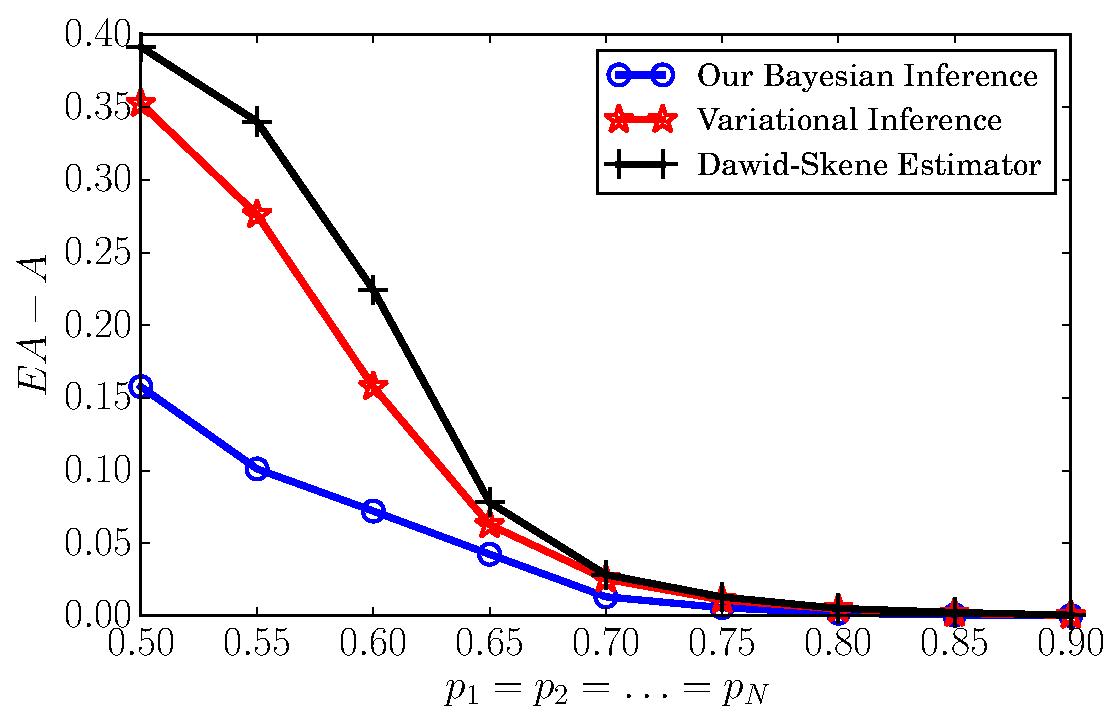
\includegraphics[width=0.45\textwidth]{image/EXPC1}
    \caption{\label{BIM}The inference bias on label accuracy}
\end{figure}

\section{Derivation of Posterior Distribution}
It is not had to figure out the joint distribution of the collected labels $\bm{L}$ and the true labels $\mathcal{L}$ 
\begin{equation*}
\label{JointDist}
\begin{split}
    &\mathbb{P}(\bm{L}, \mathcal{L}| \bm{\theta}, \bm{\tau})=\\ &\qquad {\prod}_{j=1}^{M}{\prod}_{k=1}^{2}\left\{\tau_{k}\prod_{i=1}^{N}\mathbb{P}_i^{\delta_{ijk}}(1-\mathbb{P}_i)^{\delta_{ij(3-k)}} \right\}^{\xi_{jk}}
\end{split}
\end{equation*}
where $\bm{\theta}=[\mathbb{P}_1,\ldots, \mathbb{P}_N]$ and $\bm{\tau}=[\tau_1,\tau_2]$. $\tau_1$ and $\tau_2$ denote the distribution of true label $1$ and $2$, respectively.
Besides,  $\delta_{ijk}=\mathbbm{1}(L_i(j)=k)$ and $\xi_{jk}= \mathbbm{1}(\mathcal{L}(j)=k)$.
Then, the joint distribution of $\bm{L}$, $\mathcal{L}$, $\bm{\theta}$ and $\bm{\tau}$ 
\begin{equation*}
\label{JointDist2}
\begin{split}
&\mathbb{P}(\mathcal{L},\bm{L},\bm{p}, \bm{\tau})=\mathbb{P}(\mathcal{L},\bm{L}|\bm{p}, \bm{\tau})\cdot \mathbb{P}(\bm{\theta}, \bm{\tau})\\
&=\frac{1}{B(\bm{\beta})}\prod_{k=1}^{K}\tau_k^{\hat{\beta}^{*}_k-1}\cdot\prod_{i=1}^{N}\frac{1}{B(\bm{\alpha})}p_i^{\hat{\alpha}^{*}_{i1}-1}(1-p_i)^{\hat{\alpha}^{*}_{i2}-1}
\end{split}
\end{equation*}
where $B(x,y)=(x-1)!(y-1)!/(x+y-1)!$ denotes the beta function, and
\begin{equation*}
\begin{split}
&\hat{\alpha}^{*}_{i1}={\sum}_{j=1}^{M}{\sum}_{k=1}^{K}\delta_{ijk}\xi_{jk}+\alpha_{1}\\
&\hat{\alpha}^{*}_{i2}={\sum}_{j=1}^{M}{\sum}_{k=1}^{K}\delta_{ij(3-k)}\xi_{jk}+\alpha_{2}\\
&\hat{\beta}^{*}_k={\sum}_{j=1}^{M}\xi_{jk}+\beta_{k}.
\end{split}
\end{equation*}
In this case, we can conduct marginalization via integrating the joint distribution $\mathbb{P}(\mathcal{L},\bm{L},\bm{p}, \bm{\tau})$ over $\bm{\theta}$ and $\bm{\tau}$ as
\begin{equation}
\label{marginalization}
\begin{split}
P(\mathcal{L},\bm{L}|\bm{\alpha}, \bm{\beta})=\frac{B(\hat{\bm{\beta}})}{B(\bm{\beta})}\cdot {\prod}_{i=1}^{N}\frac{B(\hat{\bm{\alpha}}_{i})}{[B(\bm{\alpha})]^2}
\end{split}
\end{equation}
where $\hat{\bm{\alpha}}_i=[\hat{\alpha}^{*}_{i1}+\alpha_1-1,\hat{\alpha}^{*}_{i2}+\alpha_2-1]$ and $\hat{\bm{\beta}}=[\hat{\beta}^{*}_1+\beta_1-1,\hat{\beta}^{*}_2+\beta_1-1]$. Following Bayes' theorem, we can know that
\begin{equation}
\label{PostDist}
P(\bm{L}|\mathcal{L})=\frac{P(\mathcal{L},\bm{L}|\bm{\alpha}, \bm{\beta})}{P(\mathcal{L}|\bm{\alpha}, \bm{\beta})}\propto B(\hat{\bm{\beta}})\prod_{i=1}^{N}B(\hat{\bm{\alpha}}_{i}). 
\end{equation}


\bibliographystyle{icml2018}
\bibliography{ref}

\end{document}


% This document was modified from the file originally made available by
% Pat Langley and Andrea Danyluk for ICML-2K. This version was created
% by Iain Murray in 2018. It was modified from a version from Dan Roy in
% 2017, which was based on a version from Lise Getoor and Tobias
% Scheffer, which was slightly modified from the 2010 version by
% Thorsten Joachims & Johannes Fuernkranz, slightly modified from the
% 2009 version by Kiri Wagstaff and Sam Roweis's 2008 version, which is
% slightly modified from Prasad Tadepalli's 2007 version which is a
% lightly changed version of the previous year's version by Andrew
% Moore, which was in turn edited from those of Kristian Kersting and
% Codrina Lauth. Alex Smola contributed to the algorithmic style files.
